
\documentclass[12pt]{article}
\setlength{\oddsidemargin}{0in}
\setlength{\evensidemargin}{0in}
\setlength{\textwidth}{6.5in}
\setlength{\parindent}{0in}
\setlength{\parskip}{\baselineskip}

\usepackage{amsmath,amsfonts,amssymb}
\usepackage{hyperref}
\usepackage[export]{adjustbox}
\usepackage{subcaption}
\usepackage{lipsum,multicol}

\title{CIS 545 - Final Project}
\author{Peter Kong}

\begin{document}

\maketitle



\hrulefill

\section{Abstract} We attack an existing authorship identification task, focusing on textual feature extraction paired with exploration in feedforward neural network classifiers.

\section{Problem Background}
Authorship identification is the task of identifying the authorship of a document, usually by textual analysis. This task has significant real world applications: it can be used to attribute authorship to historical documents whose provenance is disputed.

Many authors, with good or bad intentions, attempt to frustrate identification via various methods, including style modification [Brennan]. Helping hide or reveal authorship of text can save a life or solve a crime, depending on the context.

Authorship identification and its analog tasks are studied heavily in academia. PAN, a digital forensics conference, holds an authorship identification-related task every year. 


\section{Problem Description}
The Spooky Author Identification task is hosted by Kaggle. It is a supervised learning problem. Training data is given as tuples of (text, label), where 'text' is a one-sentence excerpt from an author's corpus, and 'label' is one of Edgar Allen Poe, H. P. Lovecraft, and Mary Wollstonecraft Shelley.

The official task tracks logless as its only metric:
\vskip 0.3in
\centerline{logloss = $-\frac{1}{N}\Sigma^N_{i=1}\Sigma^M_{j=1}y_{ij}log(p_{ij})$} 

where $M$ are the authorship classes and $y_{ij}$ is 1 if the prediction is true and 0 if it is not.

We decided to focus instead on matching-class accuracy: 
\vskip 0.3in
\centerline{accuracy = $\frac{1}{N}\Sigma^N_{i=1}\Sigma^M_{j=1}\textbf{1}y_{ij}$}

Our motivation was 2-fold: 1) in a real-world setting, probabilistic classification may be less useful than binary, 2) accuracy was a metric that all of our models could generate.

It should be noted that academic research tends to use mean-averaged precision as the primary metric. Example: [Bagnall].

\section{Data Acquisition \& Preparation}
This is a managed task, so data acquisition was straightforward. We downloaded the training data in csv format. It is comprised of 19479 rows, including gold label.

According to convention, we split the training data into three sets:
15664 rows of training data
1958 rows of validation data
1857 rows of holdout/test data

The only data wrangling necessary was a check for null values across all columns, which returned negative. We computed simple statistics across each column to check for oddities like empty sentences or out-of-vocabulary labels.


\section{Preliminary Exploration}


Here are three examples of sentences from the three authors:

\begin{quote}mws: 'How lovely is spring As we looked from Windsor Terrace on the sixteen fertile counties spread beneath, speckled by happy cottages and wealthier towns, all looked as in former years, heart cheering and fair.'
\end{quote}

\begin{quote}'It never once occurred to me that the fumbling might be a mere mistake.'
\end{quote}

\begin{quote}'This process, however, afforded me no means of ascertaining the dimensions of my dungeon; as I might make its circuit, and return to the point whence I set out, without being aware of the fact; so perfectly uniform seemed the wall.'
\end{quote}

Can you attribute each passage? You probably cannot, unless you are intimately familiar with the books these sentences are drawn from. We needed to look at much more data to find meaninful patterns.

We first truncated the corpus slightly so that all three authors were equally weighted with 5635 rows each. This avoided data skew without meaningfully descreasing corpus size. 

We used the \texttt{nltk} stopwords list across all experiments in this project, where appropriate.

We wrote a simple tokenizer for this process, which splits on white space and standard punctuation. We ensured that our tokenizer imitated the behavior of sklearn's internal tokenizer, knowing we would probably use \texttt{sklearn.TFIDFVectorizer} later. The lexicon yielded 22847 unique tokens. Next, we generated author-specific lexicons to visualize relative word frequencies:

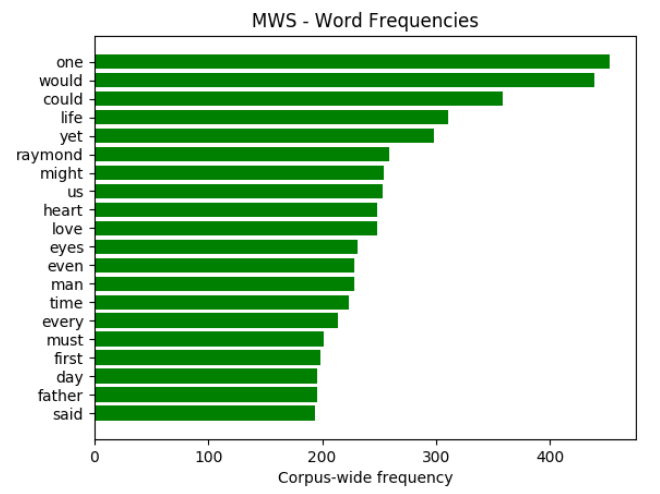
\includegraphics[scale=.40, center]{images/word_freq_mws.png}
\vskip 0.2in
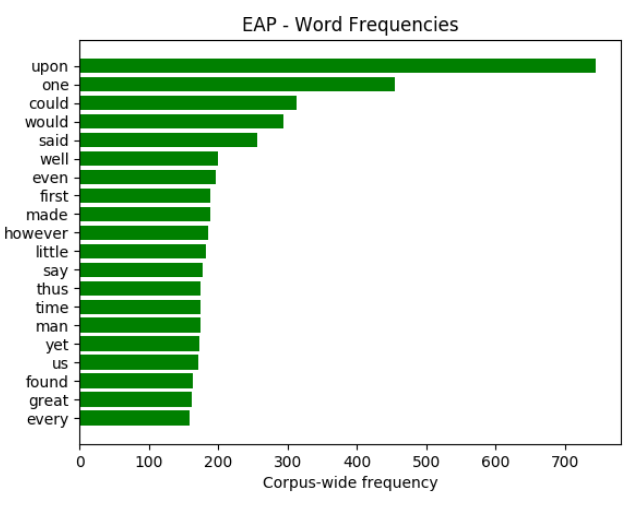
\includegraphics[scale=.40, center]{images/word_freq_eap.png}
\vskip 0.2in
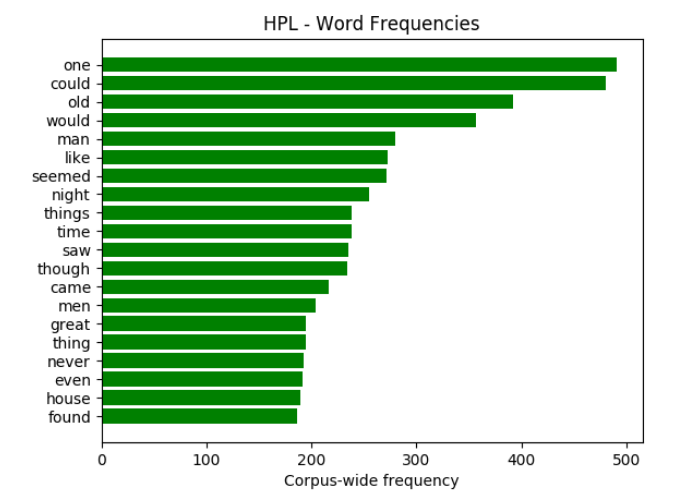
\includegraphics[scale=.40, center]{images/word_freq_hpl.png}
\vskip 0.2in

We see many commonalities - 'would', 'could', and 'man' are frequent across all authors - and many differences. This supports our intuition that word-based feature extraction techniques like TF-IDF vectorization and word embeddings will yield predictive power.

We approached this task in an iterative fashion. This, we detour into feature extraction during our exploration phase.

\section{Feature Extraction}

\subsection{TFIDF Vectorization}
TFIDF vectorization is a process that converts a chunk of text into
a fixed length set of wordwise features. Originally used for information retrieval tasks within search engines, TFIDF vectorization automatically weights words according to their relative importance (inverse document frequency) within the corpus, in theory privileging more meaningful words while ignoring noisy, common words.

The \texttt{sklearn} implementation of TFIDF vectorization allows the user to artificially limit the vocabulary used in the process, either by whitelist or by word frequency. Reducing the vocabulary reduces the degrees of freedom within the eventual model, which may in turn reduce overfit.

TFIDF vectorization is amenable to the authorship identification task because it outputs fixed length vectors for arbitrary input. One glaring shortcoming is that it can only find patterns in bags of words - it has no mechanism for observing patterns in word sequences.

Through the gridsearch technique , we found that limiting feature count to 1500

\subsection{Grammatical features}
We extracted three groups of grammatical features: punctuation, parts-of-speech ratios, and parts of speech sequences.

\begin{enumerate}
  \item Punctuation is quite straightforward. For every input, we extract the frequencies of punctuation, one feature per symbol. We used the set 
  \begin{quote} \{colon, semicolon, left parenthesis, ellipse, quote, exclamation point\}
  \end{quote} 
  We hypothesized that, since these symbols are used across a variety of domains (not just sci-fi fiction, or financial news, for example), they are likely to predict authorial style rather than content.
  \item We used the \texttt{spacy} POS tagger to label every word in our training set with it's part-of-speech tag. There is a risk that the \texttt{spacy} tagger could introduce constant biases or innacuracies since it was trained on a different distribution of text. However, it's training dataset was large and diverse enough that we took the risk.
  \\
  \texttt{spacy} produces many different tags, including relatively rare ones like interjection. We limited degrees of freedom and focused on the two parts-of-speech ratios we hypothesized had the most descriminatory power across author corpora: in-sentence adjective-to-noun ratio and adverb-to-verb ratio.
  \item So far we have only extracted bag-of-words features; we do not retain knowledge of word sequences. We created a set of sequence features by [Hearst], who in 1992 was able to leverage domain knowledge to extract semantic relationships from text using human-intuitive grammatical patterns with high accuracy. We generalize this approach by constructing one-hot POS sequence features. 

  \begin{quote}
  The fox and dog fought. \\
  NOUN\_CCONJ\_NOUN\_VERB: 1\\
  NOUN\_VERB\_NOUN\_VERB: 0\\
  ...
  \end{quote}

  Notice in the example that we severely restrict the POS tags to NOUN, VERB, CCONJ to throttle the inherent exponential growth of sequence features. Through trial and error, we found that restricting the length of POS sequence vectors to 7 limited the number of features to a reasonable 1600 without a reduction in accuracy.
\end{enumerate}

\subsection{Gensim}
We attempted to extract context-aware features a second way, through Gensim, a library that creates word2vec-style word embeddings. word2vec uses a neural network to express a given word as a vector describing its relation to neighboring words, motivated by the intuition that meaning can be recovered from a word's positional context. This technique has improved the accuracy of many NLP tasks [Mikolov]. Because we are operating at the sentence level, not word level, we used Gensim's doc2vec library, an expansion of the word2ve concept. We set vector size to 1500 to match our TFIDFVectorizer configuration.

\subsection{Named Entity Recognition}
Named Entity Recognition is a well-established research technique with high accuracy, depending on the data and domain. We ran spacy's NER extractor on our dataset. While we had hoped to find some signal from this feature set, this was the only technique we did not bother to include in our model training because of the poor results. Many sentences, like the one below, do not contain any named entities:

\begin{quote}
In whatever way the shifting is managed, it is of course concealed at every step from observation.
\end{quote}

In a basket of 1500 sentences randomly selected from our training data, we found that NER prevelence was too sparse to be helpful. Even if NER had had a better showing in our dataset, it risks predicting topic rather than author, and thus may reduce the portability of our models.

\begin{quote}
In-basket NER statistics:\\
min: 0 \\
max: 14 \\
mean: 0.8 \\
stdev: 1.2\\
\end{quote}


\section{Intermediate results}
We wanted to use neural network models to classify authorship, but first we used a simple linear classifier (\texttt{sklearn.LinearSVC}) as a way of quickly determining the value of our engineered features. (See Table 1)
\vskip 0.2in
\begin{table}[h]
  \centering
  \begin{tabular}{|l|l|}
    \hline
    Featureset  & Val. set accuracy \\
    \hline
    TFIDF      & \textbf{.558} \\
    TFIDF + 23 grammatical      & .549 \\ 
    23 grammatical      & .403 \\    
    23 grammatical + 1600 seq     & .396 \\  
    gensim (100)      & .447 \\  
    \hline
  \end{tabular}
  \caption{LinearSVC accuracy with various featuresets}
  \label{tab:sparseresults}
\end{table}

\section{Further Exploration and Data Visualization}
Somewhat dissappointingly, our engineered features performed worse than the TFIDF vectors. We visualize the data to see why this might be. Full size images can be found in Appendix. Some 'count' features have negative values - this is due to a normalization process we performed on all grammatical features to avoid favoring high-valued features:

\begin{quote}
$ normalize(x_i) = \frac{x - \bar{x}}{stdev(x)} $
\end{quote}

where $x$ is a column and $x_i$ is a single instance.
\vskip 0.2in
\begin{figure}[h]
  \begin{multicols}{3}
      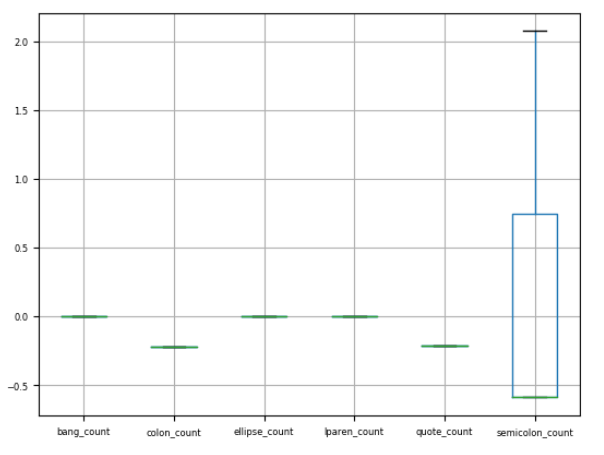
\includegraphics[width=\linewidth]{images/punc_mws.png}\par\caption{MWS}
      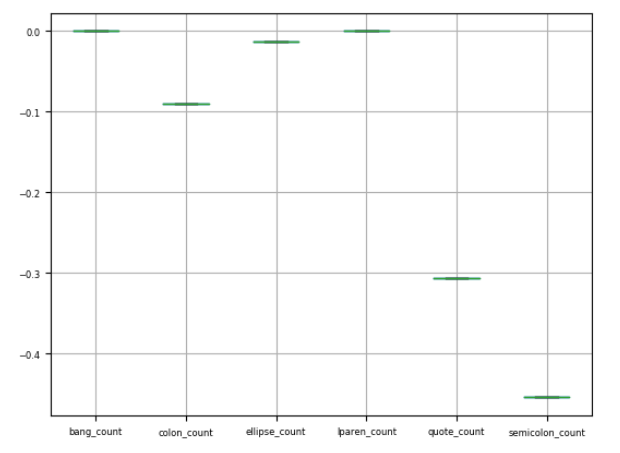
\includegraphics[width=\linewidth]{images/punc_hpl.png}\par\caption{HPL}
      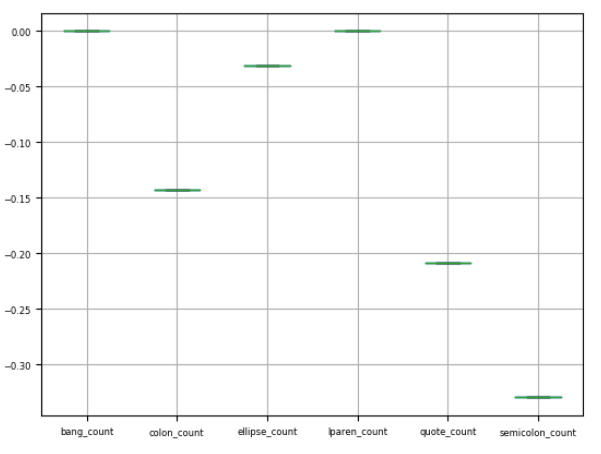
\includegraphics[width=\linewidth]{images/punc_eap.png}\par\caption{EAP}
  \end{multicols} 

  \caption{Authorwise comparison of punctuation frequencies (normalized)}
  \label{fig:punc}

\end{figure}

We observe that there punctuation counts are surprisingly consistent across all three authors, which explains why these features did not improve classification.
\vskip 0.2in
\begin{figure}[h]
  \begin{multicols}{3}
      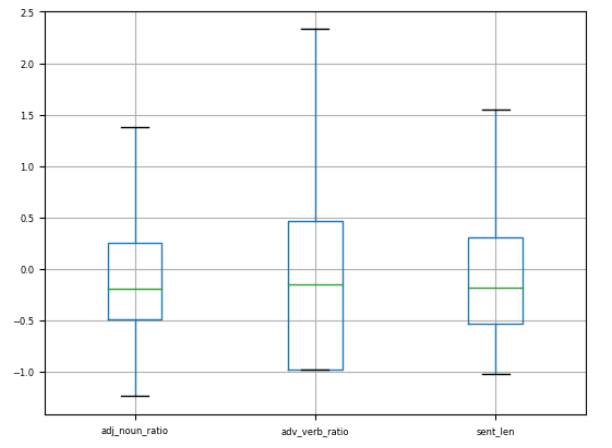
\includegraphics[width=\linewidth]{images/ratio_mws.png}\par\caption{MWS}
      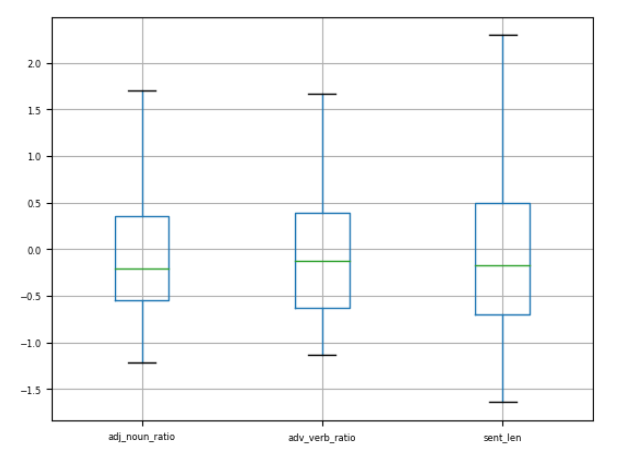
\includegraphics[width=\linewidth]{images/ratio_hpl.png}\par\caption{HPL}
      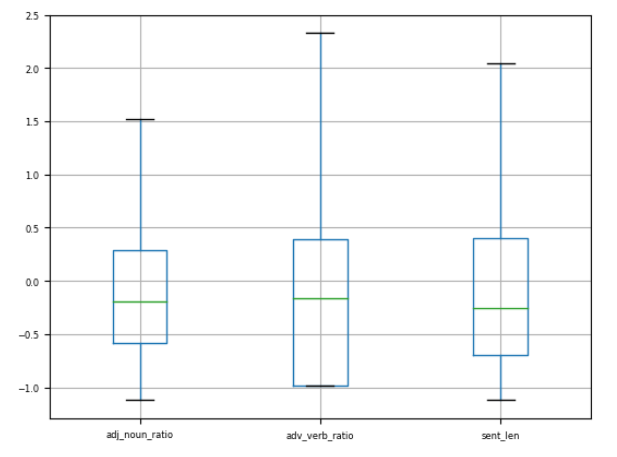
\includegraphics[width=\linewidth]{images/ratio_eap.png}\par\caption{EAP}
  \end{multicols} 

  \caption{Authorwise comparison of ratio frequencies \& sentence lengths (normalized)}
  \label{fig:punc}

\end{figure}

Likewise with ratio features and sentence length: the pattern looks similar across the three authors. EAP and MWS have higher adverb-verb variance than HPL, but the means are not substantially different.


\begin{figure}[h]
  \begin{multicols}{3}
      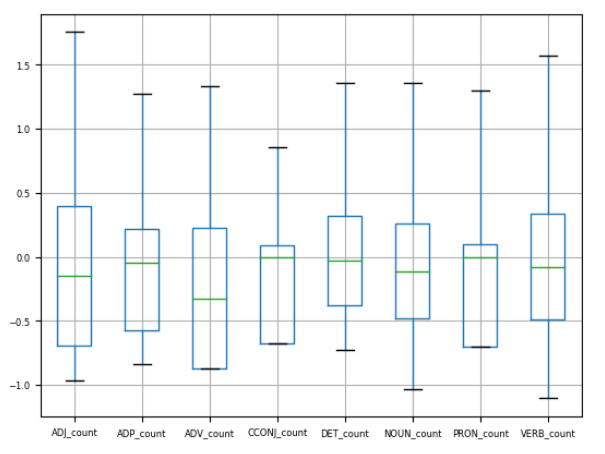
\includegraphics[width=\linewidth]{images/tag_mws.png}\par\caption{MWS}
      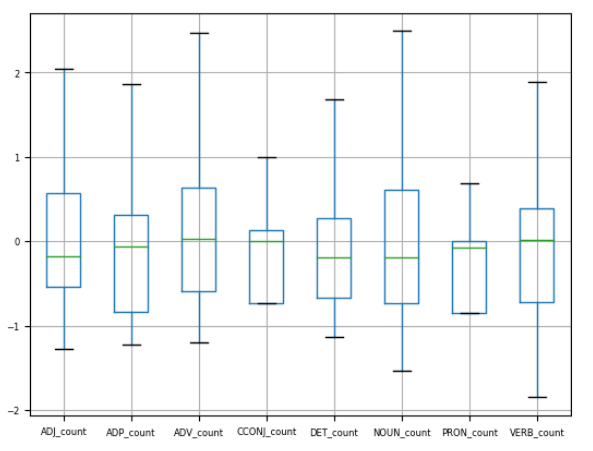
\includegraphics[width=\linewidth]{images/tag_hpl.png}\par\caption{HPL}
      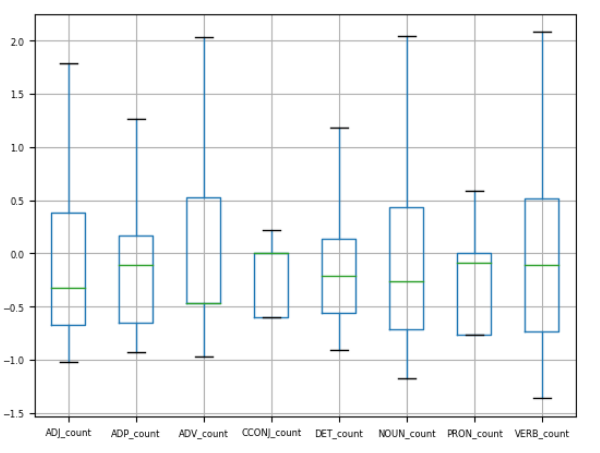
\includegraphics[width=\linewidth]{images/tag_eap.png}\par\caption{EAP}
  \end{multicols} 

  \caption{Authorwise comparison of POS frequencies (normalized)}
  \label{fig:punc}

\end{figure}

The distributions of parts-of-speech are quite similar across authors as well. Adjective and adverb frequences vary more than the other parts-of-speech, but not by much.

We can attempt to explain the engineered feature performances in three ways: 1) the engineered features, although guided by domain knowledge, are poor in carrying the signal of authorship; other, untried features should be used. 2) The corpora come from similar distributions, so there is not much signal to be noticed. 3) The LinearSVC classifier is not properly configured.


\section{NN Implementation \& Results}
After using a preliminary linear classifier for exploration, we construct 3 feedforward neural network classifiers. Each final layer was a 3-class softmax activation.
  \vskip 0.2in
  \begin{table}[h]
    \centering
    \begin{tabular}{|l|l|l|l|l|l|}
      \hline
      name & algorithm & dense layers & activation & regularization & loss \\
      \hline
      NN1 & RMS & 3 & ReLU & none & cat. crossentropy    \\
      NN2 & RMS & 5 & ReLU & l1, l2 & cat. crossentropy    \\
      NN3 & Grad. Descent & 5 & ReLU & l1, l2 & cat. crossentropy    \\
      \hline
    \end{tabular}
    \caption{NN models}
    \label{tab:nn_desc}
  \end{table}

Although the linear classifier performed poorly on most of the engineered features, we introduce them into this section, since we hypothesize that, not being confined to a linear decision boundary, the NN may be able to extract more signal from them. 

Since running a grid search on every combination of 1623 features is intractible, we group them logically into:

\begin{quote}
  gram: 23 grammatical features, 1600 sequential one-hot POS features\\
  tfidf: 1500 TFIDF features\\
  gensim: 1500 gensim features\\
\end{quote}

We established a baseline model using NN1 and all four feature groups. Then, we retrain from scratch, leaving one feature group out each time.
\vskip 0.2in
\begin{table}[h]
  \centering
  \begin{tabular}{|l|l|}
    \hline
    Featureset  & Val. set accuracy \\
    \hline
    all      & .707 \\
      - gram  & \textbf{.729} \\
      - tfidf & .553 \\
      - gensim  & .703 \\
    \hline
  \end{tabular}
  \caption{NN1 accuracy with various featuresets, epoch=10}
  \label{tab:nn1-featuresets}
\end{table}
\vskip 0.2in
Keeping the best featureset combination constant (all - gram), we retrained NN1 with different epochs:


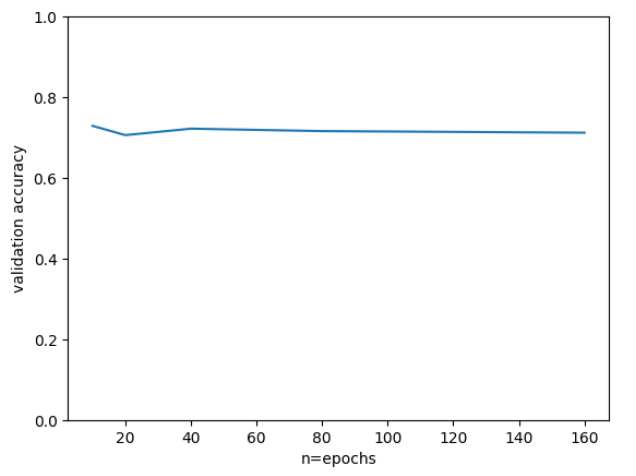
\includegraphics[scale=.45, center]{images/epochs.png}

No significant increase in accuracy was gained when increasing the number of epochs. Multiple runs of with the same NN configuration resulted in an accuracy variance of roughly 1\%.

These are our NN model results in their best configurations:

\begin{table}[h]
  \centering
  \begin{tabular}{|l|l|}
    \hline
    name & Val. set accuracy \\
    \hline
    NN1      & .729 \\
    NN2      & \textbf{.732} \\
    NN3      & .585 \\
    \hline
  \end{tabular}
  \caption{NN1 accuracy with various featuresets, epoch=10}
  \label{tab:nn-results}
\end{table}



\section{Error Analysis}
NN2 performed the best with 73.2\% accuracy. The added regularized layers controlled the final weight matrix such that it slightly outperformed its counterparts. Hold-out test set accuracy was only slightly lower, at 72.0\%.

As mentioned in the previous section, overfit was not a serious problem for the neural classifiers. Mispredictions occurred fairly evenly between classes, although NN2's most common problem was misclassifying HPL as EAP. Literature fans may find this somewhat surprising, since, Lovecraft and Poe were both American, while Shelley was English.

% Poe January 19, 1809 – October 7, 1849), boston
% Shelley  30 August 1797 – 1 February 1851) London
% Lovecraft (August 20, 1890 – March 15, 1937) rhode island

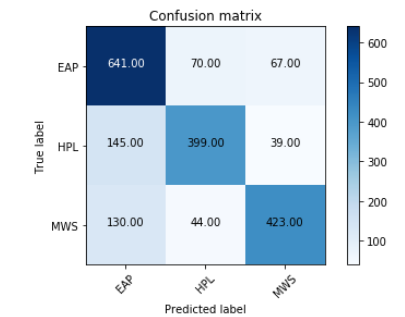
\includegraphics[scale=.45, center]{images/conf_mat.png}

In this project, we focused on feedforward neural networks. Recurrent and convolutional neural networks have shown promising results [Hu]. Many of our intuitions about feature engineering did not lead to appreciable improvements in the core metric.


%sequential, language models, LSTM

\section{Bibliography}


[Abbasi] Applying authorship analysis to extremist-group Web forum messages. \url{https://ieeexplore.ieee.org/abstract/document/1512002} \\ \\

[Bagnall] Authorship clustering using multi-headed recurrent
neural networks. \url{https://www.uni-weimar.de/medien/webis/events/pan-16/pan16-papers-final/pan16-author-identification/bagnall16-notebook.pdf}\\ \\

[Brennan] Practical Attacks Against Authorship Recognition Techniques. \url{https://www.aaai.org/ocs/index.php/IAAI/IAAI09/paper/viewFile/257/1017}\\ \\

[Hearst] Automatic Acquisition of Hyponyms
from Large Text Corpora. \url{http://people.ischool.berkeley.edu/~hearst/papers/coling92.pdf}\\ \\

[Hu] Convolutional Neural Network Architectures for
Matching Natural Language Sentences. \url{http://papers.nips.cc/paper/5550-convolutional-neural-network-architectures-for-matching-natural-language-sentences.pdf}\\ \\


[Mikolov] Efficient Estimation of Word Representations in
Vector Space. \url{https://arxiv.org/pdf/1301.3781.pdf}




\section{Appendix - Full-size plots}

\subsection{Punctuation Frequencies: MWS, HPL, EAP}
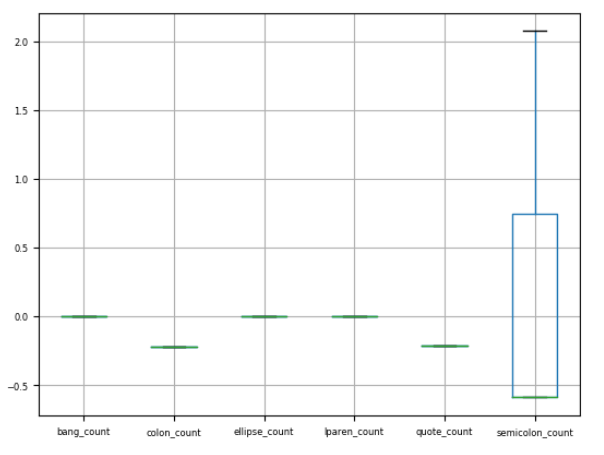
\includegraphics[scale=.50, center]{images/punc_mws.png}
\vskip 0.2in
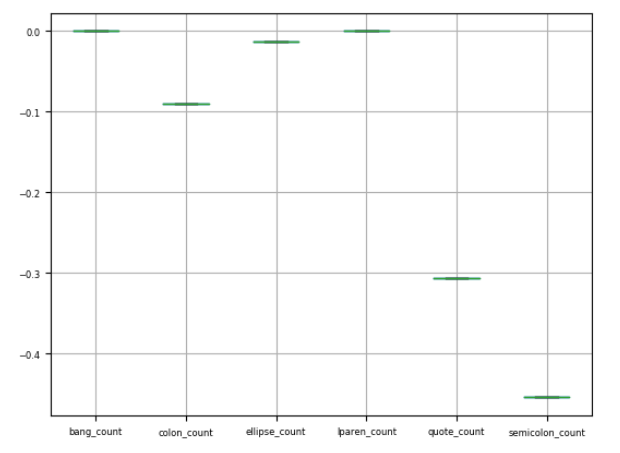
\includegraphics[scale=.50, center]{images/punc_hpl.png}
\vskip 0.2in
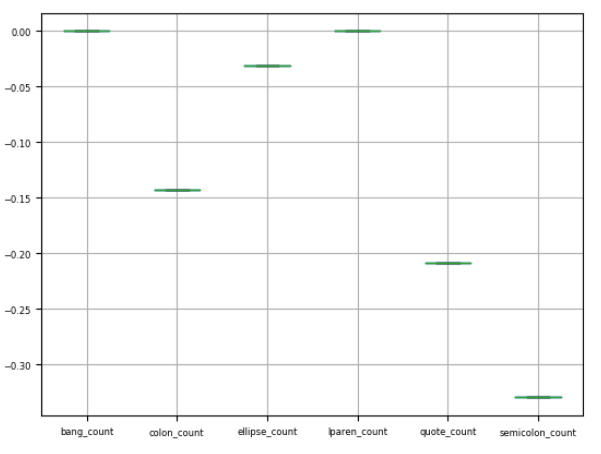
\includegraphics[scale=.50, center]{images/punc_eap.png}

\subsection{Ratios \& Sentence Length: MWS, HPL, EAP}
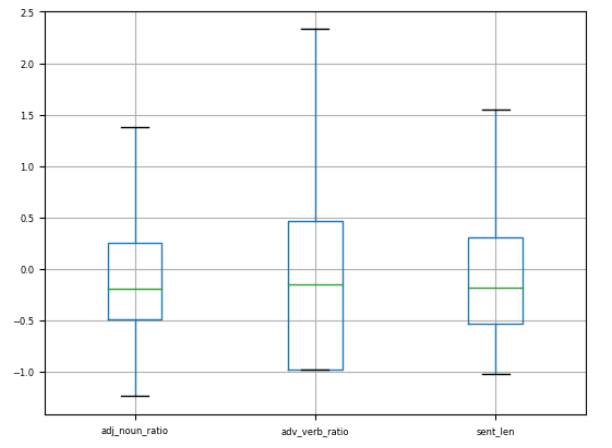
\includegraphics[scale=.50, center]{images/ratio_mws.png}
\vskip 0.2in
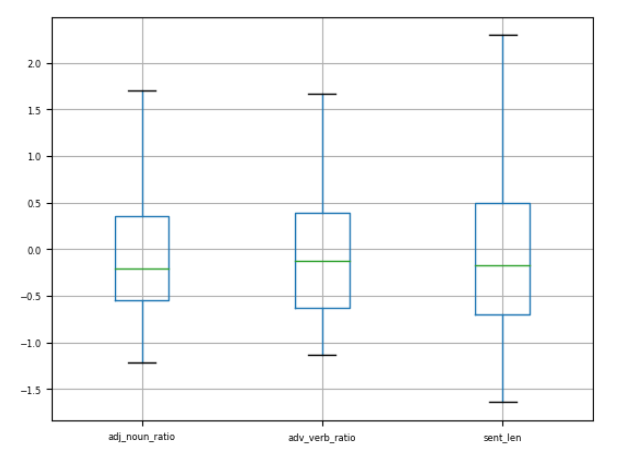
\includegraphics[scale=.50, center]{images/ratio_hpl.png}
\vskip 0.2in
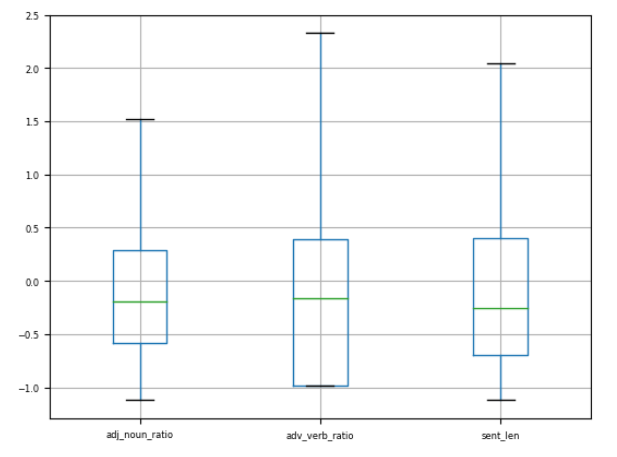
\includegraphics[scale=.50, center]{images/ratio_eap.png}



\end{document}
